\documentclass[12pt]{article}
\usepackage{amsmath}
\usepackage{graphicx}
\begin{document}
\title{Computer Science M151B, Homework 4}
\date{April 30th, 2018}
\author{Michael Wu\\UID: 404751542}
\maketitle

\section*{Problem 1}

\paragraph{a)}

The first program has
\[\frac{1.1 \text{ s} \times\frac{1 \text{ cycle}}{10^{-9} \text{ s}}}{10^9\text{ instructions}}\approx 1.1 \text{ CPI}\]
and the second has
\[\frac{1.5 \text{ s} \times\frac{1 \text{ cycle}}{10^{-9} \text{ s}}}{1.2\times 10^9\text{ instructions}}\approx 1.25 \text{ CPI}\]

\paragraph{b)}

Changing the processor means that both the cycles per instruction could change and the clock speed could change, so we cannot make any conclusions
about the relative clock speeds of the different processors.

\paragraph{c)}

The new compiler will generate an executable with the execution time
\[\frac{6\times 10^8 \text{ instructions} \times 1.1 \text{ CPI}}{10^9 \text{ cycles/s}} = 0.66 \text{ s}\]
which represents a
\[\frac{1.1\text{ s}}{0.66\text{ s}}\approx 1.667\]
times speedup over compiler A's program, and a
\[\frac{1.5\text{ s}}{0.66\text{ s}}\approx 2.273\]
times speedup over compiler B's program.

\section*{Problem 2}

\begin{align*}
        \frac{1}{10.1}&=\frac{1}{x}\times\frac{1}{2.45}\\
        x&=\frac{10.1}{2.45}\\
        x&\approx 4.122
\end{align*}
The programmer's instruction count is improved by a factor of approximately \(4.122\) relative to the compiler's.

\section*{Problem 3}

We need to find the total number of cycles over the total number of instructions.
Let \(r\) be the clock rate in cycles per second. Then the total number of instructions \(i\) is given by
\[i=r\left(\frac{3.8\text{ s}}{3\text{ CPI}}+\frac{8.5\text{ s}}{3.5\text{ CPI}}\right)=r\frac{388}{105}\text{ instructions}\]
and the total number of cycles \(c\) is given by
\[c=r(3.8\text{ s}+8.5\text{ s})=r\frac{123}{10}\text{ cycles}\]
Then we have that the new cycles per instruction will be
\[\frac{r\frac{123}{10}\text{ cycles}}{r\frac{388}{105}\text{ instructions}}\approx 3.329 \text{ CPI}\]

\section*{Problem 4}

\paragraph{a)}

Let \(i\) be the number of instructions in the program. The cycles per instruction \(x\) of non floating point operations is given by
\begin{align*}
        \frac{0.82i\times x+0.18i\times 5.3\text{ CPI}}{i}&=3.6\text{ CPI}\\
        x&\approx 3.227 \text{ CPI}
\end{align*}
Then the overall cycles per instruction for the improved processor is
\[\frac{0.82i\times 3.227+0.18i\times 3\text{ CPI}}{i} \approx 3.186\text{ CPI}\]

\paragraph{b)}

It would take \(194.7\text{ s}\) to execute the program on the improved processor.

\section*{Problem 5}

\paragraph{a)}

I would add an instruction memory unit so that the final step of load and store can be done in parallel with the instruction fetch. The last
state of both the load and store instructions would point to the instruction decode step, reducing the cycles per instruction by 1.

\begin{figure}[!ht]
    \begin{center}
        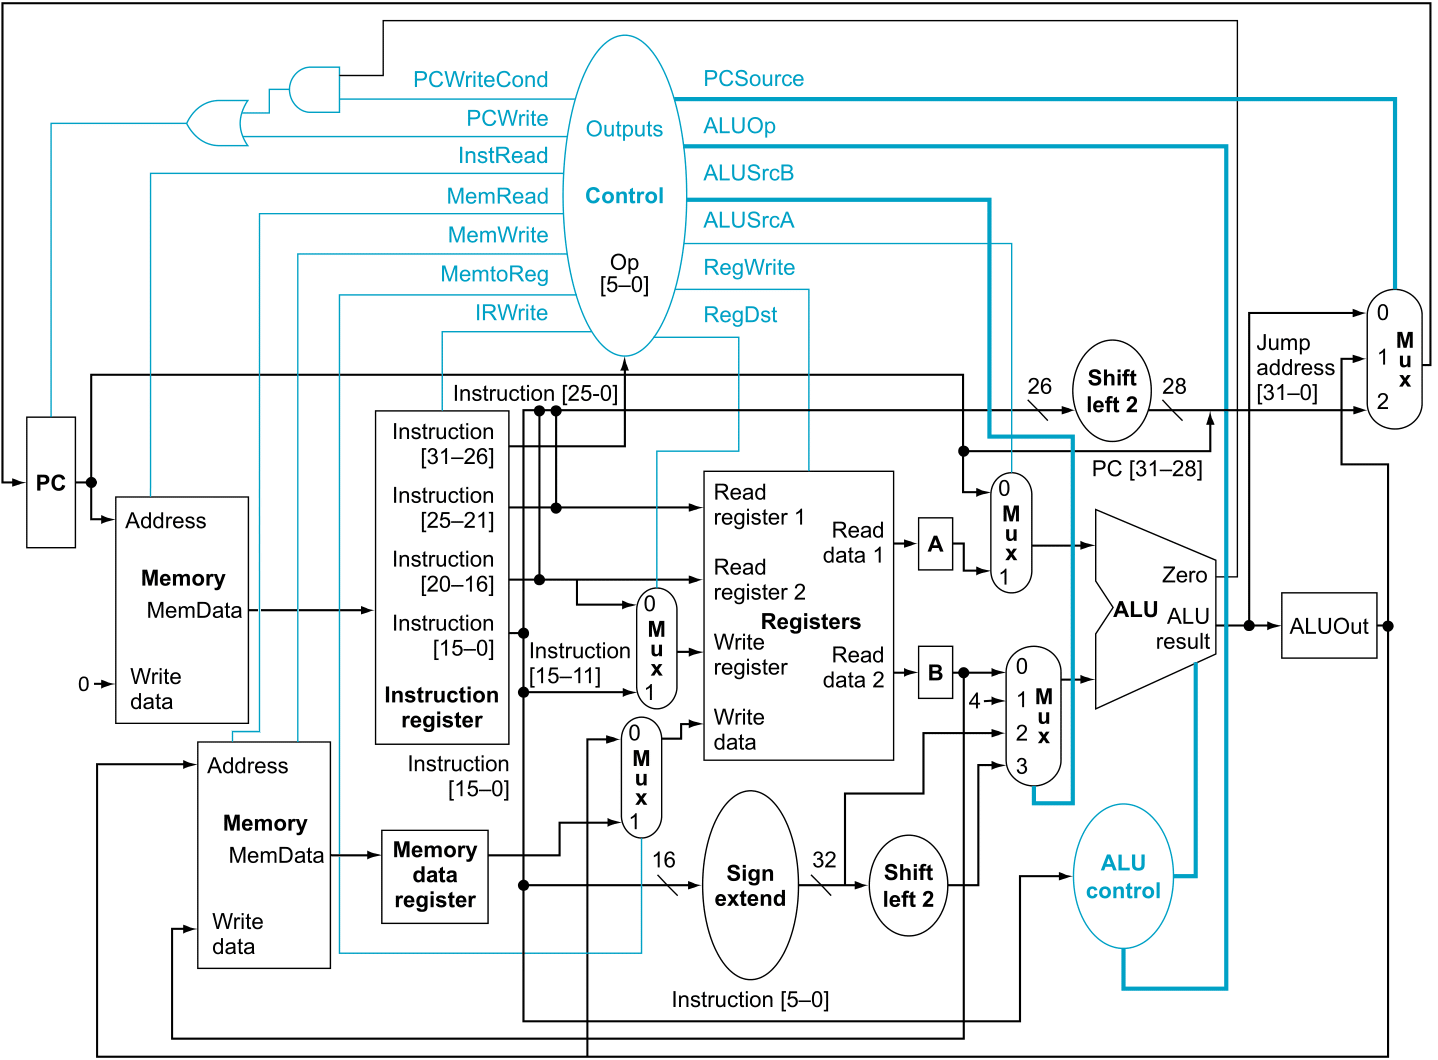
\includegraphics[width=4.8in]{problem5b.png}
    \end{center}
\end{figure}

\paragraph{b)}

The datapath changes above show the addition of the instruction memory unit. I input a zero to the \texttt{write data} signal of the instruction memory
unit since it should not be doing any writing, so this value will never be used.

\paragraph{c)}

The control signal \texttt{IorD} is renamed to \texttt{InstRead}, since there is no need for a multiplexer to choose between reading instruction memory or
regular memory. This signal controls whether to read from the address stored in the program counter or not.

\begin{figure}[!ht]
    \begin{center}
        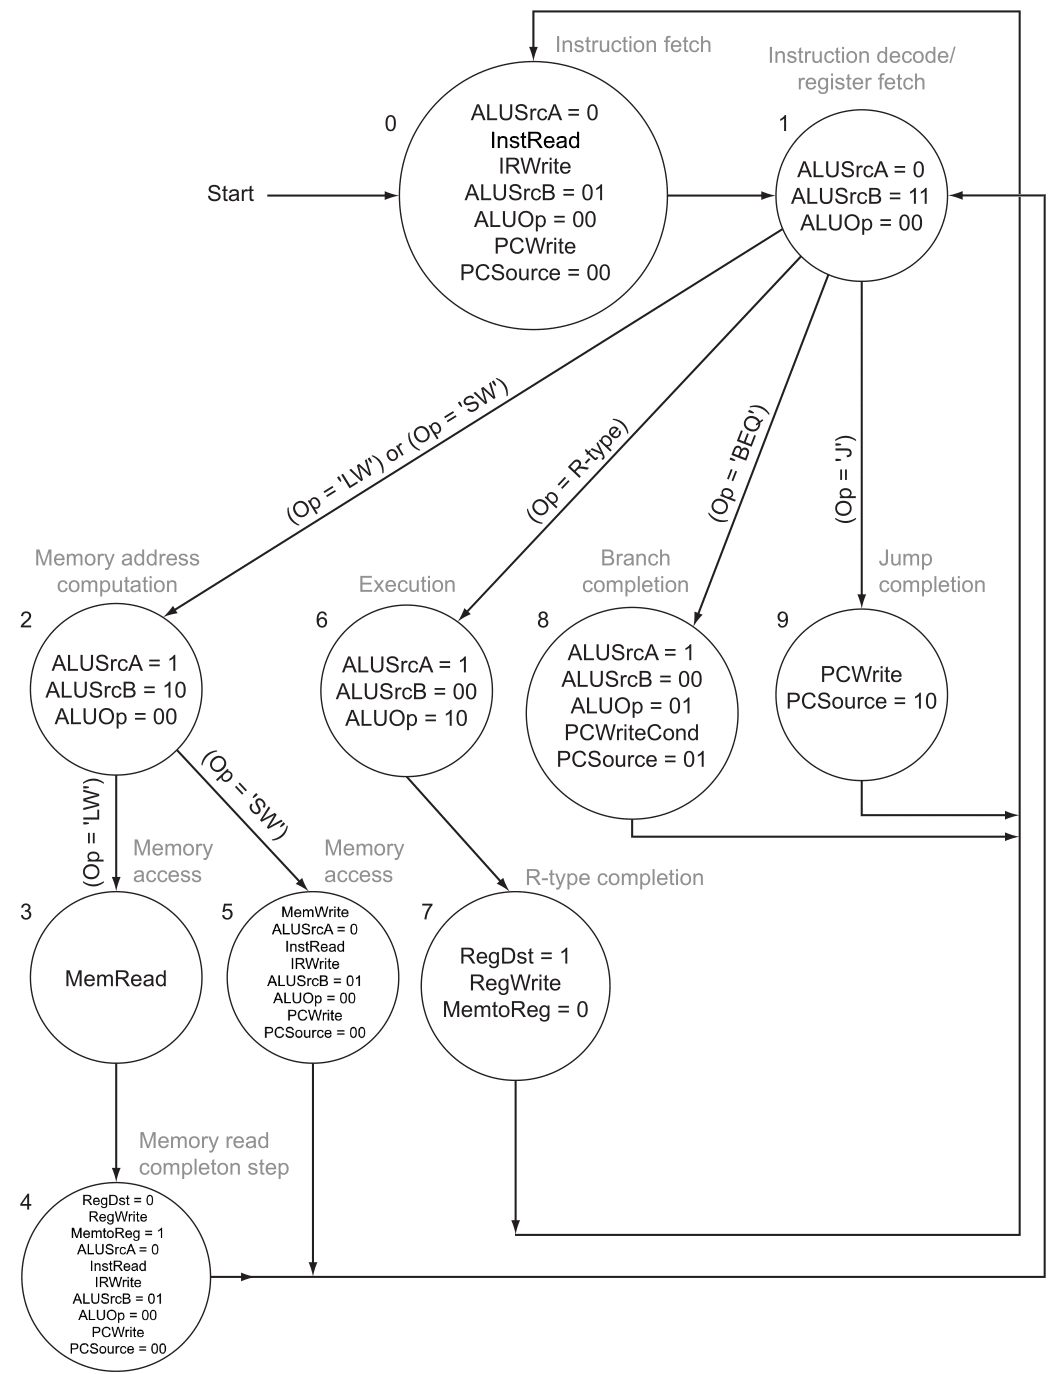
\includegraphics[width=4.7in]{problem5d.png}
    \end{center}
\end{figure}

\paragraph{d)}

The state changes are shown above. I have removed \texttt{IorD} and have allowed for the instruction fetch to happen at the same time as the last states
of the load and store instructions. This allows them to immediately go to the instruction decode step, reducing the number of cycles required by 1.

\section*{Problem 6}

\section*{Problem 7}

\section*{Problem 8}

\section*{Problem 9}

\section*{Problem 10}

\section*{Problem 11}

\end{document}